\documentclass[
	USenglish,
	aspectratio=43,
	color={accentcolor=1c},
	logo=true,
	colorframetitle=true,
	hyperref={pdfpagelabels=true},
]{tudabeamer}

% Core Packages.
\usepackage[USenglish]{babel}
\usepackage[T1]{fontenc}
\usepackage[utf8]{inputenc}
% Math Packages.
\usepackage{amsthm}
\usepackage{amsfonts}
\usepackage{amsmath}
\usepackage{amssymb}
\usepackage{mathtools}
\usepackage{bm}
\usepackage{bbm}
\usepackage{physics}
\usepackage{siunitx}
% Other Packages.
\usepackage{booktabs}
\usepackage{csquotes}
\usepackage{eqparbox}
\usepackage{datetime}
\usepackage{multimedia}
\usepackage{multicol}
\usepackage{multirow}
\usepackage{pgfplots}
\usepackage{subcaption}
\usepackage{tikz}
\usepackage{tikzscale}
% TikZ Libraries.
\usetikzlibrary{calc, arrows.meta, positioning}

% Style Definitions.
\mode<presentation>
\MakeOuterQuote{"}
\captionsetup{labelformat=empty}
\tikzset{> = { Latex[length = 2mm] }}
\mathtoolsset{showonlyrefs, showmanualtags}
\colorlet{pastelGreen}{TUDa-3c}
\colorlet{pastelBlue}{TUDa-2b}
\colorlet{pastelOrange}{TUDa-7c}
\newcommand{\ifincludelegend}[1]{}
\renewcommand{\hat}[1]{\widehat{#1}}
\renewcommand{\tilde}[1]{\widetilde{#1}}

\renewcommand{\vec}[1]{\bm{#1}}
\newcommand{\mat}[1]{\bm{\mathrm{#1}}}

\newcommand{\E}{\mathbb{E}}
\newcommand{\given}{\,\vert\,}
\newcommand{\biggiven}{\,\big\vert\,}
\newcommand{\Biggiven}{\,\Big\vert\,}
\newcommand{\bigggiven}{\,\bigg\vert\,}
\newcommand{\Bigggiven}{\,\Bigg\vert\,}
\newcommand{\PeReLU}{\ReLU_{\periodic}}
\newcommand{\periodic}{\bm{\circlearrowright}}
\newcommand{\R}{\mathbb{R}}
\newcommand{\superdagger}{\textsuperscript{$\dagger$}}
\newcommand{\transposed}{{\!\top\!}}
\newcommand{\V}{\mathbb{V}}
\newcommand{\Z}{\mathbb{Z}}

\DeclareMathOperator{\cov}{cov}
\DeclareMathOperator{\ReLU}{ReLU}

\AtBeginSection{
	\begin{frame}{\insertsectionhead \\ {\small Outline}}
		\tableofcontents[currentsection]
	\end{frame}
}
\AtBeginSubsection{
	\begin{frame}{\insertsubsectionhead \\ {\small Outline}}
		\tableofcontents[currentsection, currentsubsection]
	\end{frame}
}

\newcommand{\hypOne}{
	\begin{block}{Central Hypothesis}
		Do random Fourier series features outperform random Fourier features?
	\end{block}
}
%\newcommand{\hypTwo}{
%	\begin{block}{Hypothesis 2}
%		How do different amplitude initializations affect the performance?
%	\end{block}
%}

\newcommand{\acs}[1]{#1}
\newcommand{\acsp}[1]{#1s}
% TODO: Replace file extensions for final version.
\newcommand{\imageResultsGpCosineRfsf}     {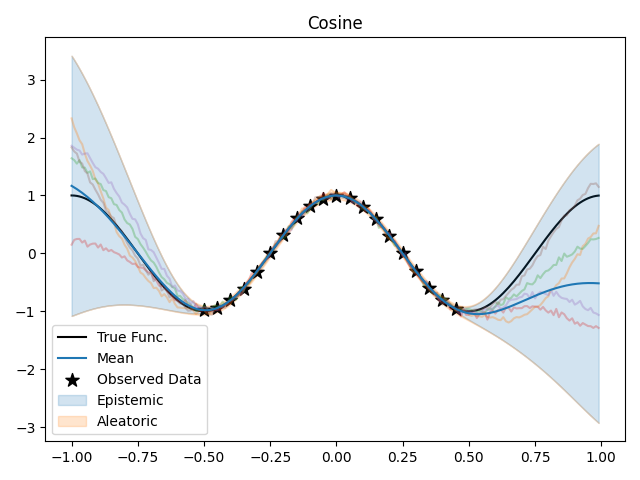
\includegraphics[width=\linewidth, height=0.618033988749895\linewidth]{graphics/generated/gp-cosine-rfsf.tikz}}
\newcommand{\imageResultsGpCosineRbf}      {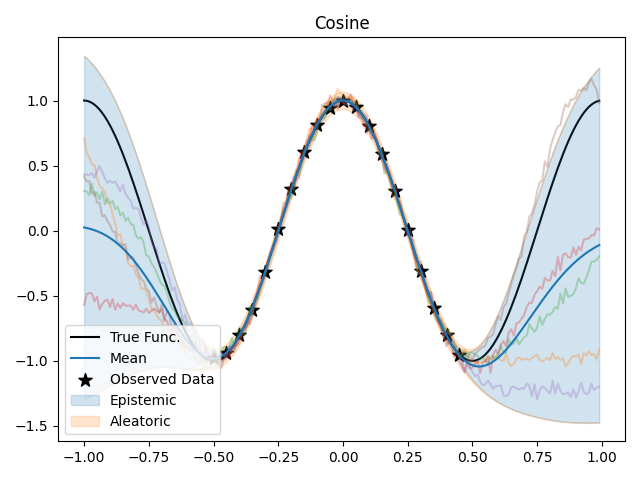
\includegraphics[width=\linewidth, height=0.618033988749895\linewidth]{graphics/generated/gp-cosine-rbf.tikz}}
\newcommand{\imageResultsGpCosineRff}      {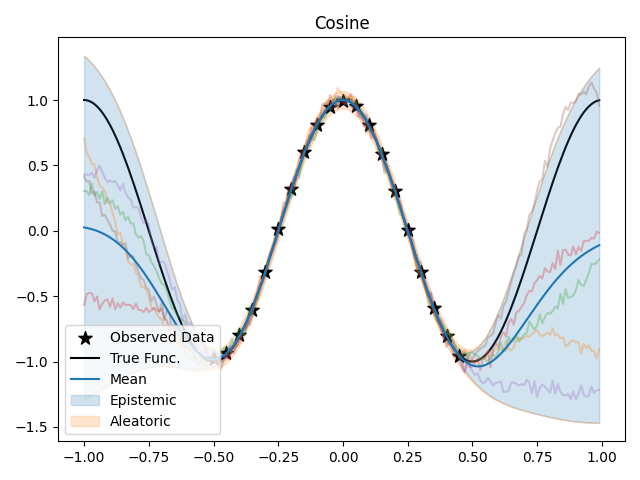
\includegraphics[width=\linewidth, height=0.618033988749895\linewidth]{graphics/generated/gp-cosine-rff.tikz}}
\newcommand{\imageResultsGpHeavisideRfsf}  {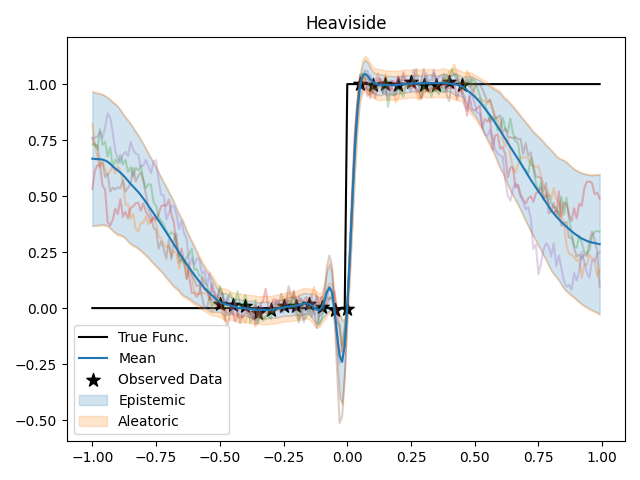
\includegraphics[width=\linewidth, height=0.618033988749895\linewidth]{graphics/generated/gp-heaviside-rfsf.tikz}}
\newcommand{\imageResultsGpHeavisideRbf}   {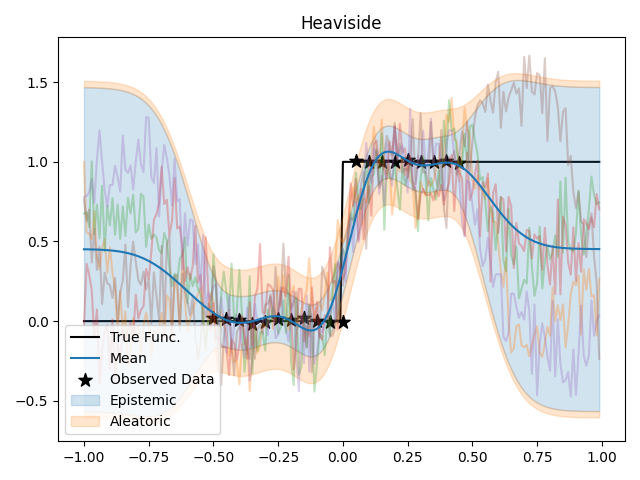
\includegraphics[width=\linewidth, height=0.618033988749895\linewidth]{graphics/generated/gp-heaviside-rbf.tikz}}
\newcommand{\imageResultsGpHeavisideRff}   {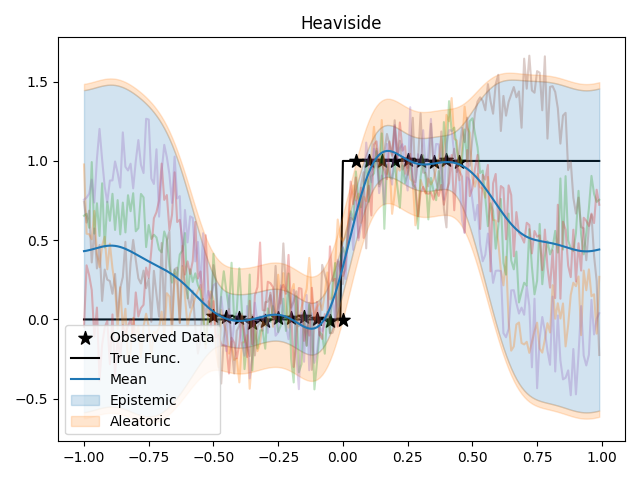
\includegraphics[width=\linewidth, height=0.618033988749895\linewidth]{graphics/generated/gp-heaviside-rff.tikz}}
\newcommand{\imageResultsGpHeavicosineRfsf}{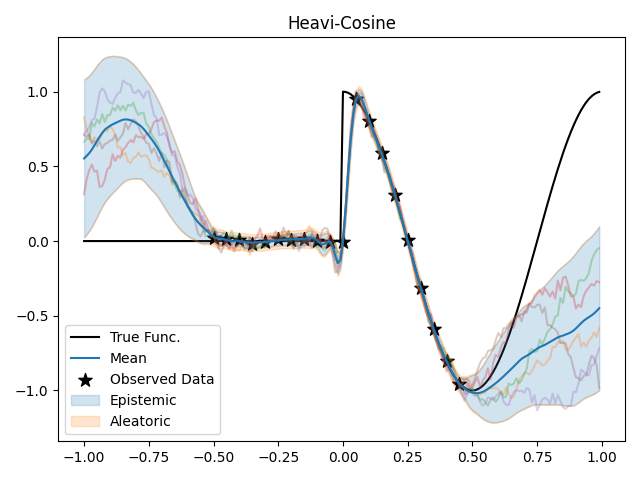
\includegraphics[width=\linewidth, height=0.618033988749895\linewidth]{graphics/generated/gp-heavicosine-rfsf.tikz}}
\newcommand{\imageResultsGpHeavicosineRbf} {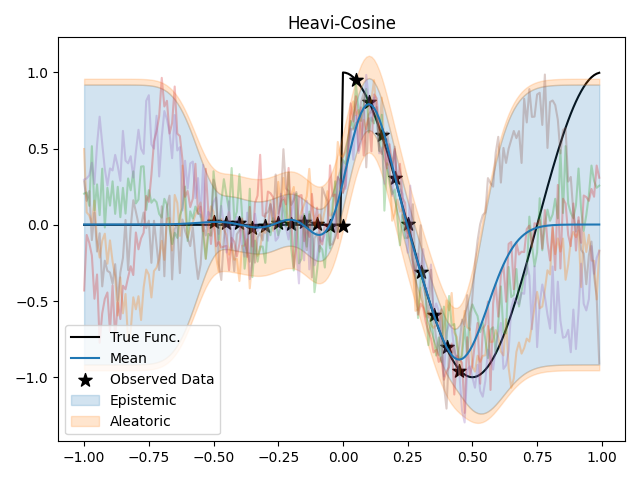
\includegraphics[width=\linewidth, height=0.618033988749895\linewidth]{graphics/generated/gp-heavicosine-rbf.tikz}}
\newcommand{\imageResultsGpHeavicosineRff} {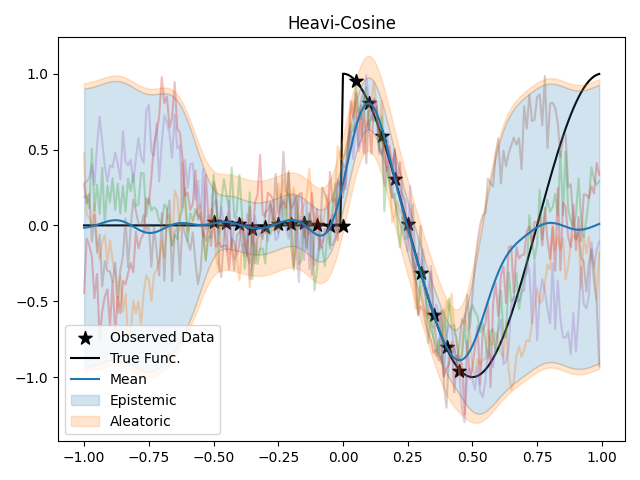
\includegraphics[width=\linewidth, height=0.618033988749895\linewidth]{graphics/generated/gp-heavicosine-rff.tikz}}
\newcommand{\imageResultsGpGapcosineRfsf}  {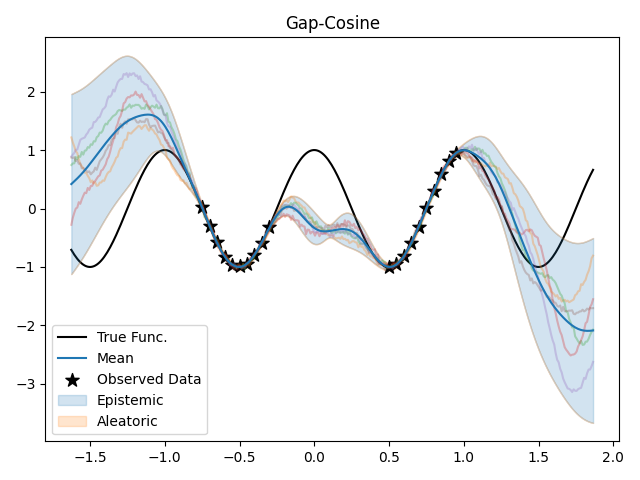
\includegraphics[width=\linewidth, height=0.618033988749895\linewidth]{graphics/generated/gp-gapcosine-rfsf.tikz}}
\newcommand{\imageResultsGpGapcosineRbf}   {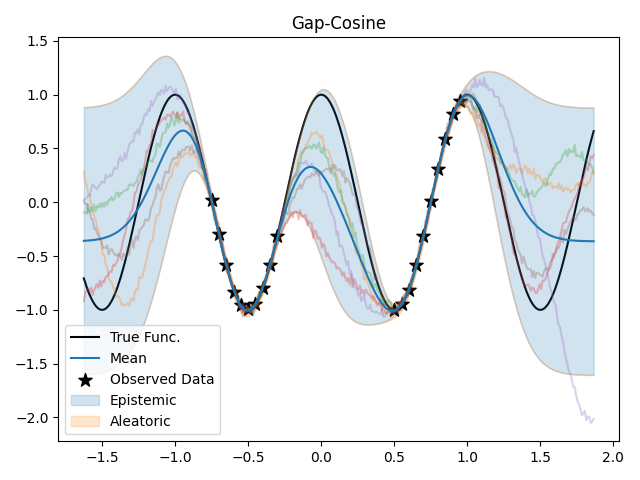
\includegraphics[width=\linewidth, height=0.618033988749895\linewidth]{graphics/generated/gp-gapcosine-rbf.tikz}}
\newcommand{\imageResultsGpGapcosineRff}   {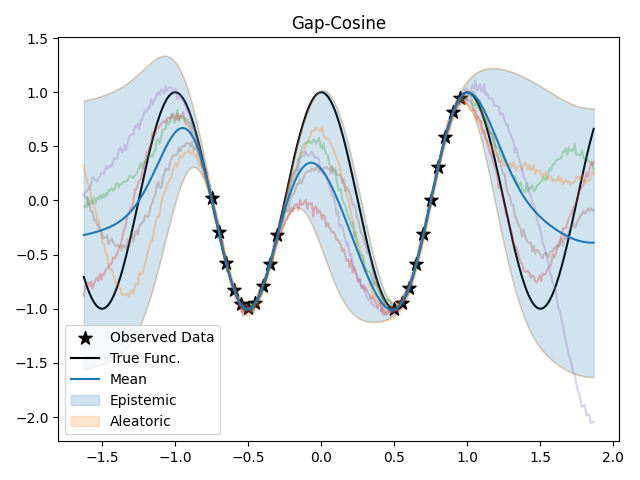
\includegraphics[width=\linewidth, height=0.618033988749895\linewidth]{graphics/generated/gp-gapcosine-rff.tikz}}


\newcommand{\tabResultsSynthetic}{
	\scriptsize
	\begin{tabular}{c|cc|ccccc}
		\toprule
		& & & \multicolumn{5}{c}{\textbf{Data Set}} \\[1pt]
		& \multicolumn{2}{c|}{\textbf{Model}}         & Cosine                 & Heaviside              & Heavi-Cosine            & Gap-Cosine             & Cartpole                          \\
		\midrule \multirow{5}{*}{\rotatebox{90}{\textbf{Log-Lik.}}}
		& \multirow[t]{3}{*}{\acs{RFSF}} & Random     & \textbf{\texttt{2.43}} & \texttt{0.11}          & \texttt{-1.66}          & \texttt{1.27}          & \texttt{~-9.88\,±\,1.86}          \\
		&                                & \acs{ReLU} & \texttt{2.34}          & \textbf{\texttt{0.80}} & \texttt{-0.90}          & \texttt{1.50}          & \texttt{-12.30\,±\,2.31}          \\
		&                                & \acs{SH}   & \texttt{2.37}          & \textbf{\texttt{0.21}} & \texttt{-1.23}          & \texttt{1.52}          & \texttt{~-9.73\,±\,2.10}          \\
		& \multirow[t]{2}{*}{\acs{GP}}   & \acs{SE}   & \textbf{\texttt{2.44}} & \texttt{0.73}          & \textbf{\texttt{~0.77}} & \textbf{\texttt{2.58}} & \textbf{\texttt{~-3.21\,±\,1.64}} \\
		&                                & \acs{RFF}  & \textbf{\texttt{2.44}} & \texttt{0.73}          & \textbf{\texttt{~0.78}} & \textbf{\texttt{2.59}} & \texttt{~-7.38\,±\,1.94}          \\
		\midrule \multirow{5}{*}{\rotatebox{90}{\textbf{\acs{RMSE}}}}
		& \multirow[t]{3}{*}{\acs{RFSF}} & Random     & \texttt{0.45}          & \texttt{0.35}          & \texttt{~0.55}          & \texttt{0.91}          & \texttt{~~0.91\,±\,0.08}          \\
		&                                & \acs{ReLU} & \textbf{\texttt{0.39}} & \texttt{1.06}          & \texttt{~3.55}          & \texttt{1.62}          & \texttt{~~1.01\,±\,0.10}          \\
		&                                & \acs{SH}   & \texttt{0.70}          & \texttt{0.35}          & \texttt{~0.48}          & \texttt{0.75}          & \texttt{~~0.98\,±\,0.11}          \\
		& \multirow[t]{2}{*}{\acs{GP}}   & \acs{SE}   & \texttt{0.45}          & \textbf{\texttt{0.30}} & \textbf{\texttt{~0.29}} & \textbf{\texttt{0.40}} & \textbf{\texttt{~~0.77\,±\,0.07}} \\
		&                                & \acs{RFF}  & \texttt{0.45}          & \textbf{\texttt{0.31}} & \textbf{\texttt{~0.30}} & \texttt{0.42}          & \texttt{~~1.26\,±\,0.10}          \\
		\bottomrule
	\end{tabular}
}

\newcommand{\tabResultsUciJoe}{
	\scriptsize
	\begin{tabular}{c|cc|cccc}
		\toprule
		& & & \multicolumn{4}{c}{\textbf{Data Set}} \\[1pt]
		& \multicolumn{2}{c|}{\textbf{Model}}                               & Boston                           & Concrete                         & Power                            & Yacht                            \\
		\midrule \multirow{11}{*}{\rotatebox{90}{\textbf{Log-Lik.}}}
		& \multirow[t]{3}{*}{\acs{RFSF}}             & Random           & \texttt{-2.40\,±\,0.05}          & \textbf{\texttt{-2.94\,±\,0.05}} & \texttt{-2.78\,±\,0.01}          & \texttt{-0.80\,±\,0.02}          \\
		&                                            & \acs{ReLU}       & \texttt{-2.39\,±\,0.05}          & \textbf{\texttt{-2.93\,±\,0.04}} & \texttt{-2.80\,±\,0.01}          & \texttt{-0.86\,±\,0.02}          \\
		&                                            & \acs{SH}         & \texttt{-2.44\,±\,0.06}          & \textbf{\texttt{-2.94\,±\,0.05}} & \texttt{-2.78\,±\,0.01}          & \texttt{-0.83\,±\,0.02}          \\
		& \multirow[t]{2}{*}{\acs{GP}}               & \acs{SE}         & \textbf{\texttt{-2.38\,±\,0.05}} & \textbf{\texttt{-2.98\,±\,0.06}} & \texttt{-2.82\,±\,0.01}          & \texttt{-0.80\,±\,0.02}          \\
		&                                            & \acs{RFF}        & \texttt{-2.40\,±\,0.06}          & \textbf{\texttt{-3.01\,±\,0.05}} & \texttt{-2.84\,±\,0.01}          & \texttt{-0.80\,±\,0.02}          \\
		& \multirow[t]{2}{*}{\acs{GBLL}}\superdagger & Leaky \acs{ReLU} & \texttt{-2.90\,±\,0.05}          & \texttt{-3.09\,±\,0.03}          & \texttt{-2.77\,±\,0.01}          & \texttt{-1.67\,±\,0.11}          \\
		&                                            & Tanh             & \texttt{-3.06\,±\,0.03}          & \texttt{-3.21\,±\,0.03}          & \texttt{-2.83\,±\,0.01}          & \texttt{-0.70\,±\,0.10}          \\
		& \multirow[t]{2}{*}{Ensemble}\superdagger   & Leaky \acs{ReLU} & \texttt{-2.48\,±\,0.09}          & \textbf{\texttt{-3.04\,±\,0.08}} & \textbf{\texttt{-2.70\,±\,0.01}} & \texttt{-0.35\,±\,0.07}          \\
		&                                            & Tanh             & \texttt{-2.48\,±\,0.08}          & \textbf{\texttt{-3.03\,±\,0.07}} & \textbf{\texttt{-2.72\,±\,0.01}} & \textbf{\texttt{-0.03\,±\,0.05}} \\
		& \multirow[t]{2}{*}{\acs{MAP}}\superdagger  & Leaky \acs{ReLU} & \texttt{-2.60\,±\,0.07}          & \texttt{-3.04\,±\,0.04}          & \texttt{-2.77\,±\,0.01}          & \texttt{-5.14\,±\,1.62}          \\
		&                                            & Tanh             & \texttt{-2.59\,±\,0.06}          & \texttt{-3.11\,±\,0.04}          & \texttt{-2.76\,±\,0.01}          & \texttt{-1.77\,±\,0.53}          \\
		\midrule \multirow{11}{*}{\rotatebox{90}{\textbf{\acs{RMSE}}}}
		& \multirow[t]{3}{*}{\acs{RFSF}}             & Random           & \textbf{\texttt{~2.95\,±\,0.15}} & \textbf{\texttt{~4.70\,±\,0.14}} & \texttt{~3.90\,±\,0.03}          & \texttt{~0.51\,±\,0.03}          \\
		&                                            & \acs{ReLU}       & \texttt{~3.51\,±\,0.44}          & \texttt{~4.77\,±\,0.15}          & \texttt{~3.95\,±\,0.04}          & \texttt{~0.53\,±\,0.03}          \\
		&                                            & \acs{SH}         & \texttt{~3.17\,±\,0.17}          & \textbf{\texttt{~4.66\,±\,0.15}} & \texttt{~3.88\,±\,0.03}          & \texttt{~0.52\,±\,0.03}          \\
		& \multirow[t]{2}{*}{\acs{GP}}               & \acs{SE}         & \textbf{\texttt{~2.81\,±\,0.12}} & \texttt{~4.98\,±\,0.15}          & \texttt{~4.03\,±\,0.03}          & \texttt{~0.51\,±\,0.04}          \\
		&                                            & \acs{RFF}        & \texttt{~2.98\,±\,0.13}          & \texttt{~5.08\,±\,0.15}          & \texttt{~4.11\,±\,0.03}          & \texttt{~0.52\,±\,0.04}          \\
		& \multirow[t]{2}{*}{\acs{GBLL}}\superdagger & Leaky \acs{ReLU} & \texttt{~4.19\,±\,0.17}          & \texttt{~5.01\,±\,0.18}          & \texttt{~3.85\,±\,0.03}          & \texttt{~1.09\,±\,0.09}          \\
		&                                            & Tanh             & \texttt{~4.61\,±\,0.23}          & \texttt{~5.50\,±\,0.23}          & \texttt{~4.09\,±\,0.04}          & \texttt{~0.43\,±\,0.03}          \\
		& \multirow[t]{2}{*}{Ensemble}\superdagger   & Leaky \acs{ReLU} & \textbf{\texttt{~2.79\,±\,0.17}} & \textbf{\texttt{~4.55\,±\,0.12}} & \textbf{\texttt{~3.59\,±\,0.04}} & \texttt{~0.83\,±\,0.08}          \\
		&                                            & Tanh             & \textbf{\texttt{~2.71\,±\,0.13}} & \textbf{\texttt{~4.51\,±\,0.13}} & \textbf{\texttt{~3.66\,±\,0.04}} & \textbf{\texttt{~0.38\,±\,0.03}} \\
		& \multirow[t]{2}{*}{\acs{MAP}}\superdagger  & Leaky \acs{ReLU} & \texttt{~3.02\,±\,0.17}          & \textbf{\texttt{~4.75\,±\,0.12}} & \texttt{~3.81\,±\,0.04}          & \texttt{~0.94\,±\,0.09}          \\
		&                                            & Tanh             & \textbf{\texttt{~3.01\,±\,0.17}} & \texttt{~5.15\,±\,0.13}          & \texttt{~3.78\,±\,0.04}          & \textbf{\texttt{~0.39\,±\,0.04}} \\
		\bottomrule
	\end{tabular}
}

\newcommand{\tabResultsUciRest}{
	\begin{tabular}{c|cc|ccccc}
		\toprule
		& & & \multicolumn{5}{c}{\textbf{Data Set}} \\[1pt]
		& \multicolumn{2}{c|}{\textbf{Model}}             & Energy                           & Kin8nm                           & Naval                                 & Protein                              & Wine                             \\
		\midrule \multirow{5}{*}{\rotatebox{90}{\textbf{Log-Lik.}}}
		& \multirow[t]{3}{*}{\acs{RFSF}} & Random         & \textbf{\texttt{-0.70\,±\,0.02}} & \texttt{~0.68\,±\,0.05}          & \texttt{~~-78.19\,±\,~69.72}          & \texttt{~~-2.94\,±\,~~0.03}          & \texttt{-0.11\,±\,0.07}          \\
		&                                & \acs{ReLU}     & \texttt{-0.74\,±\,0.02}          & \textbf{\texttt{~0.97\,±\,0.03}} & \texttt{~-172.57\,±\,104.83}          & \texttt{-629.05\,±\,384.60}          & \texttt{-0.11\,±\,0.06}          \\
		&                                & \acs{SH}       & \texttt{-0.74\,±\,0.02}          & \texttt{~0.52\,±\,0.07}          & \texttt{~~-62.69\,±\,~55.40}          & \texttt{~~-2.96\,±\,~~0.03}          & \textbf{\texttt{ 0.01\,±\,0.06}} \\
		& \multirow[t]{2}{*}{\acs{GP}}   & \acs{SE}       & \textbf{\texttt{-0.68\,±\,0.02}} & \texttt{-0.22\,±\,0.24}          & \textbf{\texttt{~~~~6.91\,±\,~~0.15}} & \textbf{\texttt{~~-2.89\,±\,~~0.00}} & \texttt{-0.84\,±\,0.05}          \\
		&                                & \acs{RFF}      & \textbf{\texttt{-0.69\,±\,0.02}} & \texttt{~0.75\,±\,0.04}          & \texttt{-1941.56\,±\,248.64}          & \texttt{~~-2.90\,±\,~~0.00}          & \texttt{-0.89\,±\,0.04}          \\
		\midrule \multirow{5}{*}{\rotatebox{90}{\textbf{\acs{RMSE}}}}
		& \multirow[t]{3}{*}{\acs{RFSF}} & Random         & \textbf{\texttt{~0.48\,±\,0.02}} & \textbf{\texttt{~0.07\,±\,0.00}} & \texttt{~~~~0.01\,±\,0.00~~}          & \textbf{\texttt{~~~3.97\,±\,0.02~~}} & \textbf{\texttt{~0.64\,±\,0.01}} \\
		&                                & \acs{ReLU}     & \textbf{\texttt{~0.49\,±\,0.02}} & \textbf{\texttt{~0.07\,±\,0.00}} & \texttt{~~~~0.01\,±\,0.00~~}          & \textbf{\texttt{~~~4.00\,±\,0.03~~}} & \texttt{~0.66\,±\,0.01}          \\
		&                                & \acs{SH}       & \textbf{\texttt{~0.49\,±\,0.02}} & \texttt{~0.08\,±\,0.00}          & \texttt{~~~~0.01\,±\,0.00~~}          & \textbf{\texttt{~~~3.97\,±\,0.02~~}} & \texttt{~0.65\,±\,0.01}          \\
		& \multirow[t]{2}{*}{\acs{GP}}   & \acs{SE}       & \textbf{\texttt{~0.48\,±\,0.02}} & \texttt{~0.08\,±\,0.00}          & \textbf{\texttt{~~~~0.00\,±\,0.00~~}} & \texttt{~~~4.34\,±\,0.01~~}          & \textbf{\texttt{~0.63\,±\,0.01}} \\
		&                                & \acs{RFF}      & \textbf{\texttt{~0.48\,±\,0.01}} & \textbf{\texttt{~0.07\,±\,0.00}} & \texttt{~~~~0.02\,±\,0.00~~}          & \texttt{~~~4.42\,±\,0.01~~}          & \textbf{\texttt{~0.63\,±\,0.01}} \\
		\bottomrule
	\end{tabular}
}


% Document Information.
\title{Random Fourier Series Features}
\subtitle{Defense \enquote{Expert Lab on Robot Learning}}
\author{Fabian Damken}
\institute{Intelligent Autonomous Systems}
\department{Department of Computer Science}
\date{\formatdate{20}{05}{2022}}

\logo*{
\includegraphics{graphics/ias-logo}}
\titlegraphic*{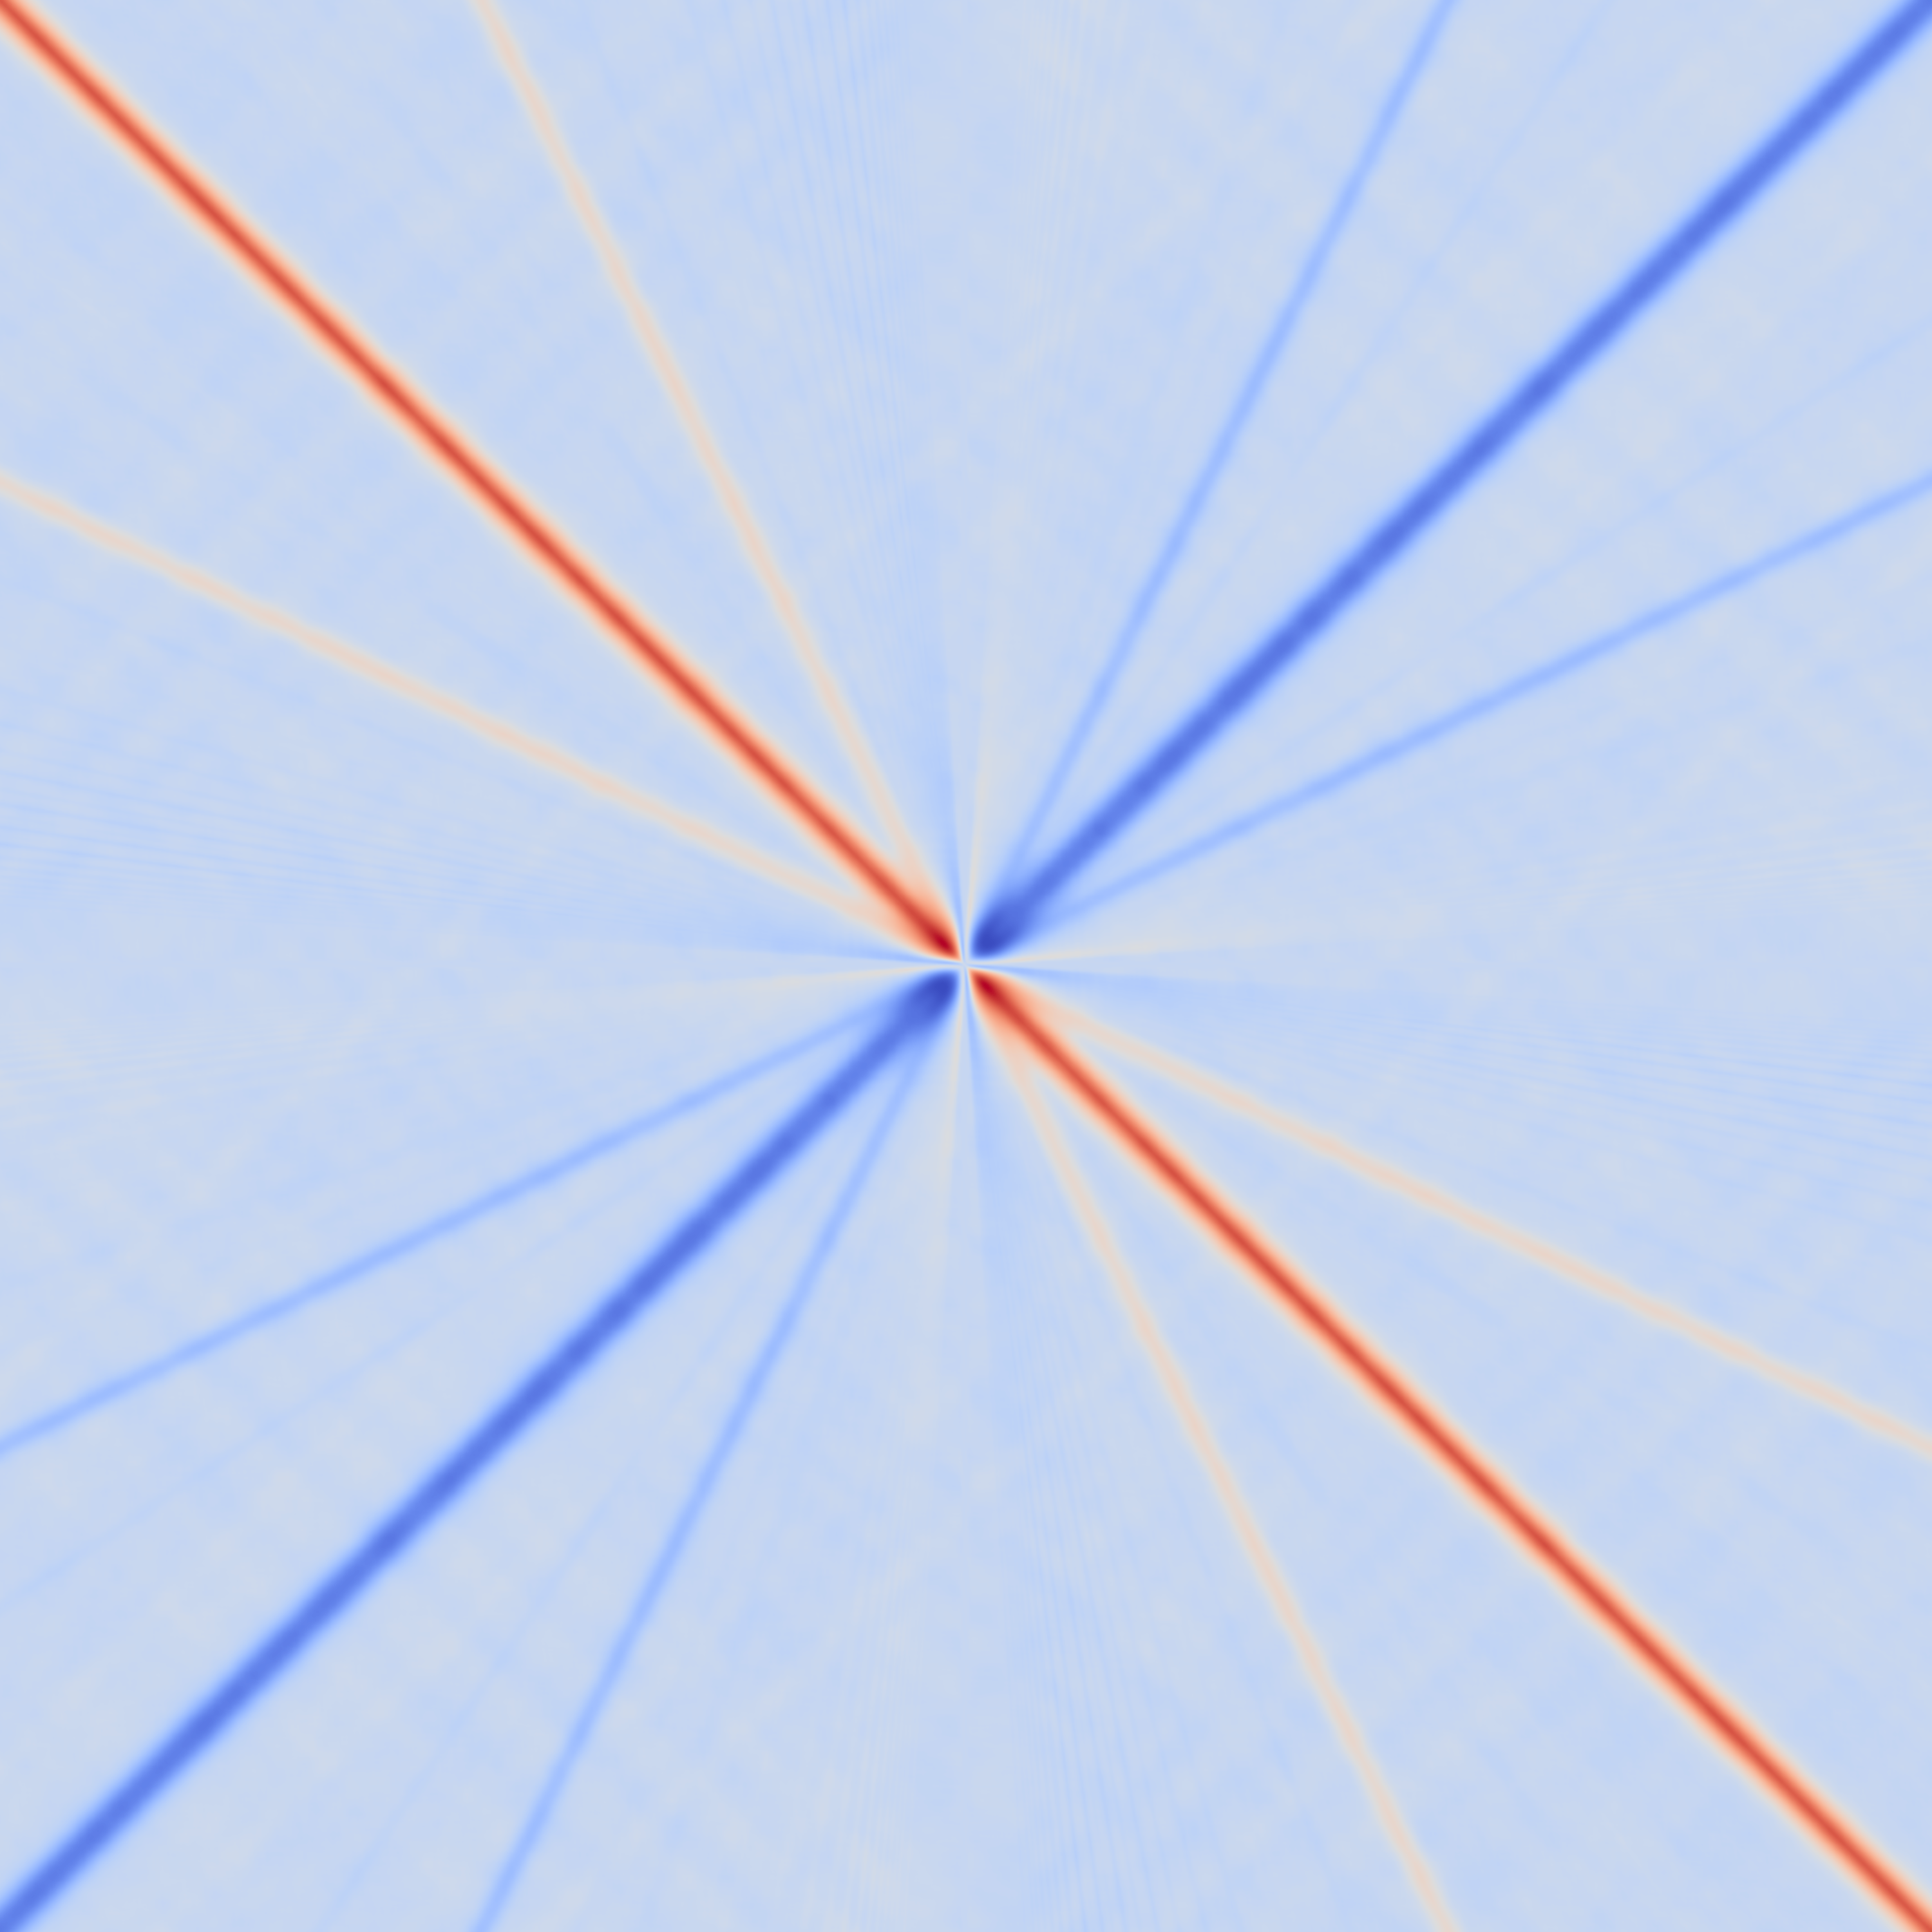
\includegraphics{graphics/generated/title}}

\begin{document}
	\maketitle

	\section{Motivation}
		\begin{frame}{Deep Learning and Neural Networks}
			\begin{itemize}
				\item<+-> (Deep) neural networks dominate AI
					\begin{itemize}
						\item<+-> extremely expressive
						\item<.-> great predictive power
						\item<+-> lack of uncertainty estimation
					\end{itemize}
				\item<+-> Lead to the development of \emph{Bayesian} neural networks
					\begin{itemize}
						\item<+-> intractable exact inference
						\item<.-> complicated training
						\item<.-> unreliable uncertainty quantification
						\item<.-> \dots
					\end{itemize}
			\end{itemize}
		\end{frame}

		\begin{frame}{Gaussian Processes (GPs)}
			\begin{itemize}
				\item<+-> GPs are still the go-to model for reliable uncertainty quantification
				\item<+-> but performance highly depends on the kernel choice\dots
				\item<.-> exact inference complexity is cubic w.r.t. number of data points
					\begin{itemize}
						\item prohibits online use of GPs
					\end{itemize}
			\end{itemize}
		\end{frame}
	% end

	\section{Methodology}
		\begin{frame}{Random Fourier Features}
			\begin{equation}
				\vec{z}_{\vec{\omega}}(\vec{x}) =
					\begin{bmatrix}
						\cos(\ip{\vec{\omega}}{\vec{x}}) \\
						\sin(\ip{\vec{\omega}}{\vec{x}})
					\end{bmatrix}
			\end{equation}
			\begin{itemize}
				\item<+-> resort to "classical" Bayesian regression
				\item<.-> explicit posterior over the weights
				\item<+-> approximate every stationary kernel \( k(\cdot) \):
			\end{itemize}
			\onslide<.->{
				\begin{gather}
					k(\vec{x} - \vec{y}) = \E_{\vec{\omega} \sim p(\cdot)}\bigl[ \ip{\vec{z}_{\vec{\omega}}(\vec{x})}{\vec{z}_{\vec{\omega}}(\vec{y})} \bigr]
				\end{gather}
			}
			\begin{itemize}
				\item<+-> for the SE, \( p(\vec{\omega}) = \mathcal{N}(\vec{\omega} \given \vec{0}, \mat{I}) \)
				\item<+-> SE kernel is extremely smooth
			\end{itemize}
		\end{frame}

		\begin{frame}{Random Fourier \emph{Series} Features}
			We extend random Fourier features:
			\begin{equation}
				\begin{aligned}
					\vec{z}_{\vec{\omega}}(\vec{x}) &=
						\begin{bmatrix}
							\cos(\ip{\vec{\omega}}{\vec{x}}) \\
							\sin(\ip{\vec{\omega}}{\vec{x}})
						\end{bmatrix}
				\end{aligned}
				\qquad\longrightarrow\qquad
				\begin{aligned}
					\vec{z}_{\vec{\omega}}(\vec{x}) &= \sum_{k = 1}^{K} \vec{z}_{\vec{\omega}}^{(k)}(\vec{x}), \\
					\vec{z}_{\vec{\omega}}^{(k)}(\vec{x}) &=
						\begin{bmatrix}
							a_k \cos(\pi \tilde{T}^{-1} k \mel{\vec{\omega}}{\bm{\Lambda}^{-1}}{\vec{x}}) \\
							b_k \sin(\pi \tilde{T}^{-1} k \mel{\vec{\omega}}{\bm{\Lambda}^{-1}}{\vec{x}})
						\end{bmatrix}
				\end{aligned}
			\end{equation}
			\begin{itemize}
				\item<+-> similar to the sine-cosine formulation of Fourier series
				\item<.-> motivated the name
			\end{itemize}
		\end{frame}

		\begin{frame}{Hyper-Parameter Optimization}
			\begin{columns}
				\begin{column}{0.5\linewidth}
					\begin{itemize}
						\item<+-> Hyper-Parameters
							\begin{itemize}
								\item \eqmakebox[hyperParams][l]{\(\vec{a}_{1:K}\)} (sine coefficients)
								\item \eqmakebox[hyperParams][l]{\(\vec{b}_{1:K}\)} (cosine coefficients)
								\item \eqmakebox[hyperParams][l]{\(\bm{\Lambda}\)}  (length-scales)
								\item \eqmakebox[hyperParams][l]{\(\tilde{T}\)}     (half-period)
								\item \eqmakebox[hyperParams][l]{\(\sigma_n^2\)}    (aleatoric noise variance)
							\end{itemize}
						\item<+-> maximization of the marginal log-likelihood
						\item<.-> using the empirical Bayes approximation
					\end{itemize}
				\end{column}
				\begin{column}{0.5\linewidth}
					\begin{align}
						\vec{z}_{\vec{\omega}}(\vec{x}) &= \sum_{k = 1}^{K} \vec{z}_{\vec{\omega}}^{(k)}(\vec{x}), \\
						\vec{z}_{\vec{\omega}}^{(k)}(\vec{x}) &=
							\begin{bmatrix}
								a_k \cos(\pi \tilde{T}^{-1} k \mel{\vec{\omega}}{\bm{\Lambda}^{-1}}{\vec{x}}) \\
								b_k \sin(\pi \tilde{T}^{-1} k \mel{\vec{\omega}}{\bm{\Lambda}^{-1}}{\vec{x}})
							\end{bmatrix}
					\end{align}
				\end{column}
			\end{columns}
		\end{frame}
	% end

	\section{Evaluation}
		\begin{frame}{Hypothesis}
			\hypOne
		\end{frame}

		\begin{frame}{Evaluation}
			\begin{itemize}
				\item<+-> Datasets:
					\begin{itemize}
						\item Synthetic Data (Cosine, Heaviside, Heavi-Cosine, Gap-Cosine)
						\item UCI (Boston, Concrete, Power, Yacht, Energy, Kin8nm, Naval, Protein, Wine)
						\item Cartpole
					\end{itemize}
				\item<+-> Different RFSF Initializations:
					\begin{itemize}
						\item Random
						\item ReLU
						\item Single Harmonic (SH)
					\end{itemize}
			\end{itemize}
		\end{frame}

		\begin{frame}{How the Kernel Learns}
			\begin{columns}
				\begin{column}{0.5\linewidth}
					\centering
					\movie[loop]{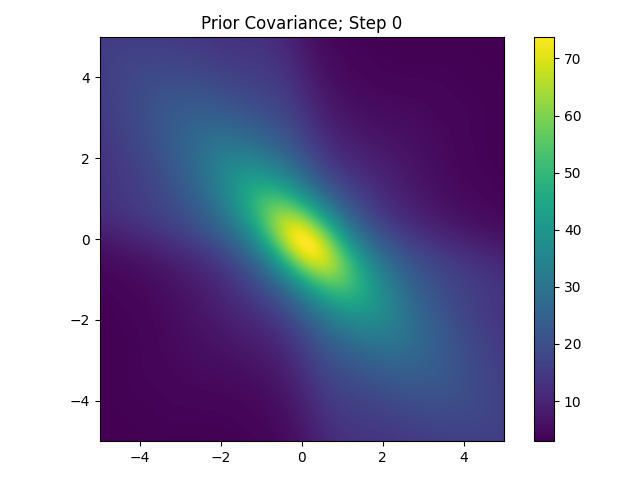
\includegraphics[width=\linewidth]{graphics/kernel-animation/rfsf/prior-covariance.png}}{graphics/kernel-animation/rfsf/prior-covariance.webm}
					RFSF on Gap-Cosine
				\end{column}
				\begin{column}{0.5\linewidth}
					\centering
					\movie[loop]{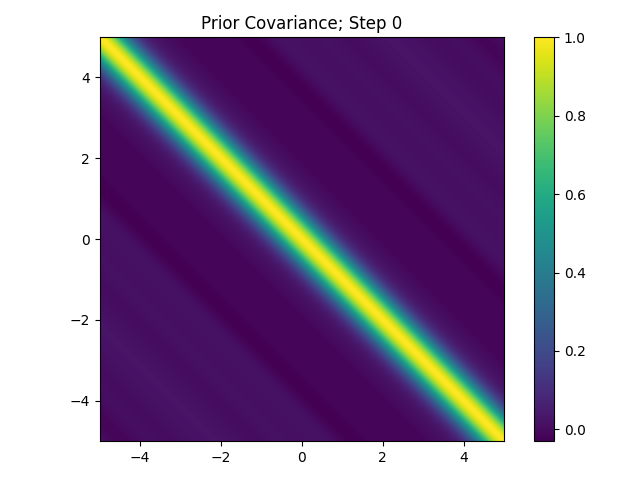
\includegraphics[width=\linewidth]{graphics/kernel-animation/rff/prior-covariance.png}}{graphics/kernel-animation/rff/prior-covariance.webm}
					RFFs on Gap-Cosine
				\end{column}
			\end{columns}
		\end{frame}

		\begin{frame}{Results on the Synthetic Data}
			\begin{center}
				\begin{tabular}{c|cc}  % TODO: Change to TikZ file extension.
					& RFSFs & RFFs \\ \midrule
					\rotatebox{90}{\parbox{0.22\linewidth}{\centering Gap-Cosine}}
					& 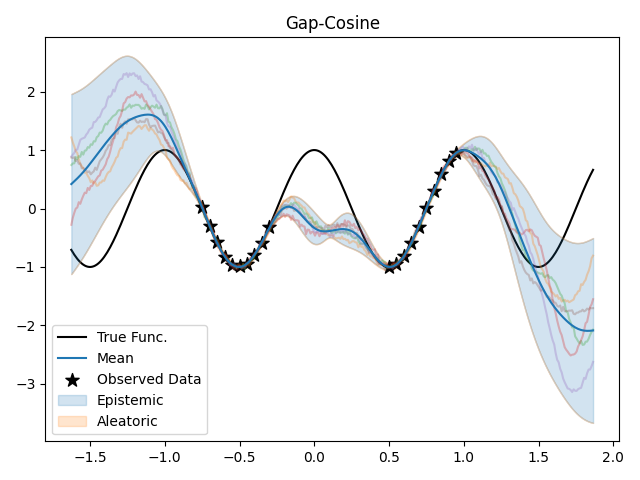
\includegraphics[width=0.4\linewidth, height=0.22\linewidth]{graphics/generated/gp-gapcosine-rfsf.png}
					& 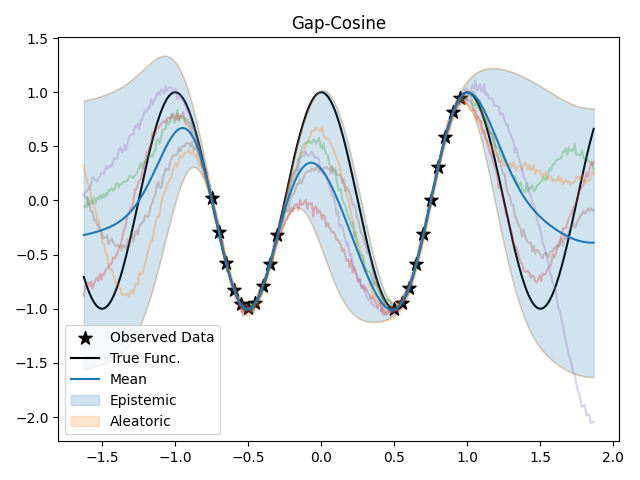
\includegraphics[width=0.4\linewidth, height=0.22\linewidth]{graphics/generated/gp-gapcosine-rff.png}
					\\
					\rotatebox{90}{\parbox{0.22\linewidth}{\centering Heavi-Cosine}}
					& 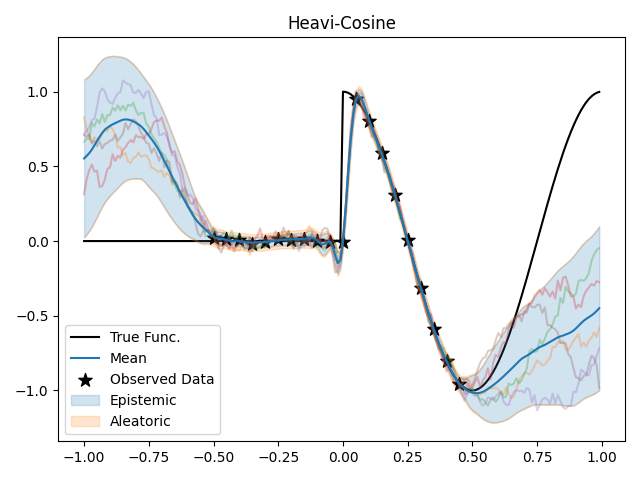
\includegraphics[width=0.4\linewidth, height=0.22\linewidth]{graphics/generated/gp-heavicosine-rfsf.png}
					& 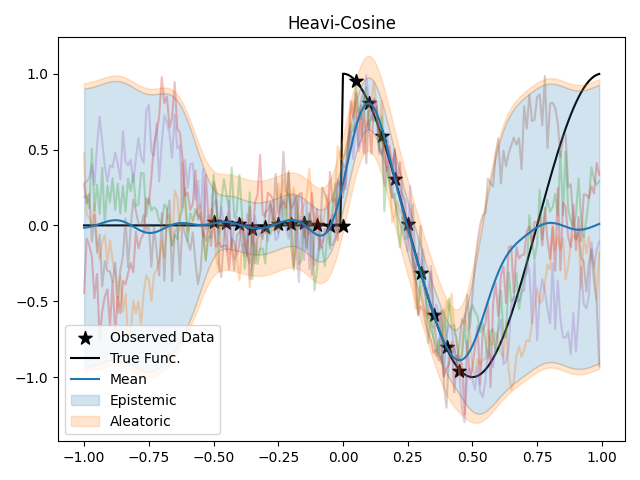
\includegraphics[width=0.4\linewidth, height=0.22\linewidth]{graphics/generated/gp-heavicosine-rff.png}
				\end{tabular}
			\end{center}
		\end{frame}

		\begingroup
		\let\scriptsize\relax
		\begin{frame}{Quantified Results}{Synthetic Data Sets and Cartpole}
			\begin{center}
				\tiny
				\tabResultsSynthetic
			\end{center}
		\end{frame}

		\begin{frame}{Quantified Results}{UCI Data Sets}
			\begin{center}
				\tiny
				\tabResultsUciJoe

				\vspace{1pt}
				\textsuperscript{\(\dagger\)}Results taken from Watson et al. (2021), "Latent Derivative Bayesian Last Layer Networks."
			\end{center}
		\end{frame}
		\endgroup
	% end

	\section{Conclusion}
		\begin{frame}{Conclusion}
			\hypOne

			\begin{itemize}
				\item<+-> compared to RFFs, SE, and BNN methods
				\item<+-> advantage of RFSFs is not consistent
				\item<.-> no performance gain
				\item<.-> also true for the SH initialization
			\end{itemize}
		\end{frame}

		\begin{frame}{Future Work}
			\begin{itemize}
				\item theoretical analysis what RFSFs approximate
				\item better understanding of the half-period initialization
			\end{itemize}
		\end{frame}
	% end


	\appendix
	\section{Evaluation}
		\begin{frame}{Quantified Results}{UCI Data Sets; Cont.}
			\begin{center}
				\tiny
				\tabResultsUciRest
			\end{center}
		\end{frame}
	% end
\end{document}
